
\begin{figure}[t!]
    \centering
    \scalebox{0.9}{
    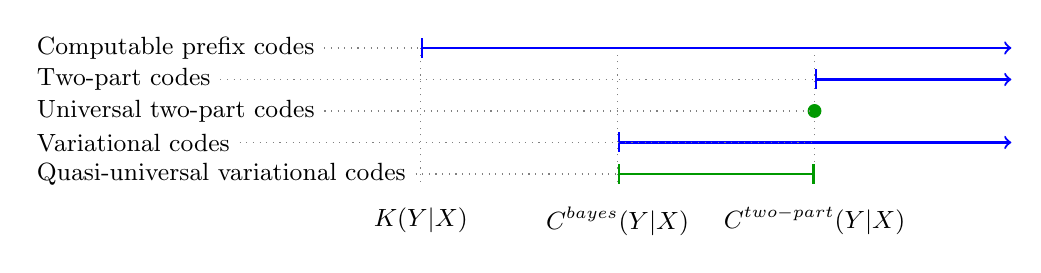
\begin{tikzpicture}[
    axis/.style={thick, ->, >=stealth},
    code_label/.style={anchor=west, font=\small},
    formula_label/.style={below=0.2cm, text width=3.5cm, text centered, font=\small},
    blue_code/.style={blue, thick},
    green_code/.style={green!60!black, thick},
    v_helper_line/.style={thin, dotted, gray},
    h_helper_line/.style={thin, dotted, gray}
]

    \def\xKYX{0}       %
    \def\xUBC{2.5}     %
    \def\xUTPC{5.0}    %
    \def\xInfinity{7.5} %
    \def\xLabelCol{-5} %
    \def\lenVar{1.5}   %

    \def\yPrefix{1.7}      %
    \def\yTwoPart{1.3}     %
    \def\yUTPC{0.9}        %
    \def\yVar{0.5}         %
    \def\yQuasi{0.1}       %


    \coordinate (kyx) at (\xKYX,0);
    \coordinate (ubc) at (\xUBC,0);
    \coordinate (utpc) at (\xUTPC,0);
    \coordinate (infinity) at (\xInfinity,0);

    \draw[v_helper_line] (ubc) -- (ubc |- 0, \yPrefix);
    \draw[v_helper_line] (kyx) -- (kyx |- 0, \yPrefix);
    \draw[v_helper_line] (utpc) -- (utpc |- 0, \yPrefix);
    
    \node[formula_label] at (kyx) {$K(Y|X)$};
    \node[formula_label] at (ubc) 
    {$C^{\text{bayes}}(Y|X)$};
    \node[formula_label] at (utpc)
        {$C^{\text{two-part}}(Y|X)$};

    
    \node[code_label] (prefix_label) at (\xLabelCol, \yPrefix) {Computable prefix codes};
    \draw[blue_code, |->] (kyx |- 0, \yPrefix) -- (infinity |- 0, \yPrefix);
    \draw[h_helper_line] (prefix_label.east) -- (kyx |- 0, \yPrefix);

    \node[code_label] (twopart_label) at (\xLabelCol, \yTwoPart) {Two-part codes};
    \draw[blue_code, |->] (utpc |- 0, \yTwoPart) -- (infinity |- 0, \yTwoPart);
    \draw[h_helper_line] (twopart_label.east) -- (utpc |- 0, \yTwoPart);

    \node[code_label] (utpc_label) at (\xLabelCol, \yUTPC) {Universal two-part codes};
    \fill[green!60!black] (utpc |- 0, \yUTPC) circle (2.5pt);
    \draw[h_helper_line] (utpc_label.east) -- (utpc |- 0, \yUTPC);

    \node[code_label] (var_label) at (\xLabelCol, \yVar) {Variational codes};
    \draw[blue_code, |->] (ubc |- 0, \yVar) -- (infinity |- 0, \yVar);
    \draw[h_helper_line] (var_label.east) -- (utpc |- 0, \yVar);

    \node[code_label] (quasi_label) at (\xLabelCol, \yQuasi) {Quasi-universal variational codes};
    \draw[green_code, |-|] (ubc |- 0, \yQuasi) -- (utpc |- 0, \yQuasi);
    \draw[h_helper_line] (quasi_label.east) -- (ubc |- 0, \yQuasi);
    
        
\end{tikzpicture}

    } %
    \caption{\textbf{Upper and lower bounds on minimum codelengths.} The figure shows the minimum number of bits required to transmit labels $Y$ given inputs $X$, for different classes of codes. The bounds hold for any dataset ($X,Y$) up to an additive constant that does not depend on the dataset.}
    \label{fig:codelength_comparisons}
\end{figure}
